\documentclass[11pt]{article} 
\usepackage[english]{babel}
\usepackage[utf8]{inputenc}
\usepackage[margin=0.5in]{geometry}
\usepackage{amsmath}
\usepackage{amsthm}
\usepackage{amsfonts}
\usepackage{amssymb}
\usepackage[usenames,dvipsnames]{xcolor}
\usepackage{graphicx}
\usepackage[siunitx]{circuitikz}
\usepackage{tikz}
\usepackage{tkz-berge}
\usetikzlibrary{positioning, automata, backgrounds}
\usepackage[colorinlistoftodos, color=orange!50]{todonotes}
\usepackage{hyperref}
\usepackage[numbers, square]{natbib}
\usepackage{fancybox}
\usepackage{epsfig}
\usepackage{soul}
\usepackage[framemethod=tikz]{mdframed}
\usepackage[shortlabels]{enumitem}
\usepackage[version=4]{mhchem}
\usepackage{multicol}
\usepackage{forest}
\usepackage{mathtools}
\usepackage{comment}
\usepackage{enumitem}
\usepackage[utf8]{inputenc}
\usepackage{listings}
\usepackage{color}
\usepackage[numbers]{natbib}
\usepackage{subfiles}
\usepackage{tkz-berge}
\usepackage{algorithm}
\usepackage[noend]{algpseudocode}


\newtheorem{prop}{Proposition}[section]
\newtheorem{thm}{Theorem}[section]
\newtheorem{lemma}{Lemma}[section]
\newtheorem{cor}{Corollary}[prop]

\theoremstyle{definition}
\newtheorem{definition}{Definition}

\theoremstyle{definition}
\newtheorem{required}{Problem}

\theoremstyle{definition}
\newtheorem{ex}{Example}

\newcommand{\interval}[4]{\draw (#2, #1) -- (#3, #1); % Usage: \interval{height}{start}{end}{label}
\draw (#2, #1-0.11) -- (#2, #1+0.11); % draw left whisker
\draw (#3, #1-0.11) -- (#3, #1+0.11); % draw right whisker
\node[] at (#2-0.25, #1) {#4};
}


\setlength{\marginparwidth}{3.4cm}
%#########################################################

%To use symbols for footnotes
\renewcommand*{\thefootnote}{\fnsymbol{footnote}}
%To change footnotes back to numbers uncomment the following line
%\renewcommand*{\thefootnote}{\arabic{footnote}}

% Enable this command to adjust line spacing for inline math equations.
% \everymath{\displaystyle}

% _______ _____ _______ _      ______ 
%|__   __|_   _|__   __| |    |  ____|
%   | |    | |    | |  | |    | |__   
%   | |    | |    | |  | |    |  __|  
%   | |   _| |_   | |  | |____| |____ 
%   |_|  |_____|  |_|  |______|______|
%%%%%%%%%%%%%%%%%%%%%%%%%%%%%%%%%%%%%%%

\title{
\normalfont \normalsize 
\textsc{CSCI 3104 Fall 2021 \\ 
Instructors: Profs. Grochow and Waggoner} \\
[10pt] 
\rule{\linewidth}{0.5pt} \\[6pt] 
\huge Problem Set 8\\
\rule{\linewidth}{2pt}  \\[10pt]
}
%\author{Your Name}
\date{}

\begin{document}
\definecolor {processblue}{cmyk}{0.96,0,0,0}
\maketitle


%%%%%%%%%%%%%%%%%%%%%%%%%
%%%%%%%%%%%%%%%%%%%%%%%%%%
%%%%%%%%%%FILL IN YOUR NAME%%%%%%%
%%%%%%%%%%AND STUDENT ID%%%%%%%%
%%%%%%%%%%%%%%%%%%%%%%%%%%
\noindent
Due Date \dotfill TODO \\
Name \dotfill \textbf{John Blackburn} \\
Student ID \dotfill \textbf{JOBL2177} \\
Collaborators \dotfill \textbf{List Your Collaborators Here}

\tableofcontents

\section{Instructions}
 \begin{itemize}
	\item The solutions \textbf{must be typed}, using proper mathematical notation. We cannot accept hand-written solutions. \href{http://ece.uprm.edu/~caceros/latex/introduction.pdf}{Here's a short intro to \LaTeX.}
	\item You should submit your work through the \textbf{class Canvas page} only. Please submit one PDF file, compiled using this \LaTeX \ template.
	\item You may not need a full page for your solutions; pagebreaks are there to help Gradescope automatically find where each problem is. Even if you do not attempt every problem, please submit this document with no fewer pages than the blank template (or Gradescope has issues with it).

	\item You are welcome and encouraged to collaborate with your classmates, as well as consult outside resources. You must \textbf{cite your sources in this document.} \textbf{Copying from any source is an Honor Code violation. Furthermore, all submissions must be in your own words and reflect your understanding of the material.} If there is any confusion about this policy, it is your responsibility to clarify before the due date. 

	\item Posting to \textbf{any} service including, but not limited to Chegg, Reddit, StackExchange, etc., for help on an assignment is a violation of the Honor Code.

	\item You \textbf{must} virtually sign the Honor Code (see Section \ref{HonorCode}). Failure to do so will result in your assignment not being graded.
\end{itemize}


\section{Honor Code (Make Sure to Virtually Sign)} \label{HonorCode}

\begin{required}
\begin{itemize}
\item My submission is in my own words and reflects my understanding of the material.
\item Any collaborations and external sources have been clearly cited in this document.
\item I have not posted to external services including, but not limited to Chegg, Reddit, StackExchange, etc.
\item I have neither copied nor provided others solutions they can copy.
\end{itemize}

%\noindent In the specified region below, clearly indicate that you have upheld the Honor Code. Then type your name. 
\end{required}

\begin{proof}[Agreed John Blackburn.]
%% Typing "I agree to the above," followed by your name is sufficient.
\end{proof}


\newpage
\section{Standard 21- Dynamic Programming: Identify the Precise Subproblems}

\noindent The goal of this standard is to practice identifying the recursive structure. To be clear, you are \textbf{not} being asked for a precise mathematical recurrence. Rather, you are being asked to clearly and precisely identify the cases to consider. Identifying the cases can sometimes provide enough information to design a dynamic programming solution.

\subsection{Problem \ref{DP1}}
\begin{required} \label{DP1}
Consider the \textsf{Stair Climbing} problem, defined as follows.
\begin{itemize}
\item \textsf{Instance:} Suppose we have $n$ stairs, labeled $s_{1}, \ldots, s_{n}$. Each stair $s_{k}$ has a number $a_{k} \geq 1$ associated to it. At stair $s_{k}$, we may jump forward $i$ stairs, where $i \in \{ 1, 2, \ldots, a_{k}\}$. You start on $s_{1}$.

\item \textsf{Solution:} The number of ways to to reach $s_{n}$ from $s_{1}$.
\end{itemize}

\noindent \\ \textbf{Your job} is to clearly identify the recursive structure. That is, suppose we are solving the subproblem at stair $s_{k}$. What precise sub-problems do we need to consider?
\end{required}

\begin{proof}[Answer]
%Your answer

The subproblems that need to be solved to solve subproblem at stair $s_k$ are as follows: we need to know the amount of paths possible to reach each stair prior to stair $s_k$. That is we need to solve the amount of paths possible to stair $s_1$ all the way up to stair $s_{k-1}$ individually, in order to solve the subproblem at stair $s_k$. If we know the amount of possible paths to each stair prior to $s_k$ we can use that information to find the amount of possible paths to stair $s_k$. 

\end{proof}



\newpage
\subsection{Problem \ref{DP2}}
\begin{required} \label{DP2}
Fix $n \in \mathbb{N}$. The \textit{Trust Game} on $n$ rounds is a two-player dynamic game. Here, Player I starts with \$100. The game proceeds as follows.
\begin{itemize}
\item \textbf{Round 1:} Player I takes a fraction of the \$100 (which could be nothing) to give to Player II. The money Player I gives to Player II is multiplied by 1.5 before Player II receives it. Player I keeps the remainder. (So for example, if Player I gives \$20 to Player II, then Player II receives \$30 and Player I is left with \$80).

\item \textbf{Round 2:} Player II can choose a fraction of the money they received to offer to Player I. The money offered to Player I increases by a multiple of $1.5$  before Player I receives it. Player II keeps the remainder.
\end{itemize}

\noindent \\ More generally, at round $i$, the Player at the current round (Player I if $i$ is odd, and Player II if $i$ is even) takes a fraction of the money in the current pile to send to the other Player and keeps the rest. That money increases by a factor of $1.5$ before the other player receives it. The game terminates if the current player does not send any money to the other player, or if round $n$ is reached. At round $n$, the money in the pile is split evenly between the two players. \\

\noindent Each individual player wishes to maximize the total amount of money they receive. \\

\noindent \textbf{Your job} is to clearly identify the recursive structure. That is, at round $i$, what precise sub-problems does the current player need to consider? [\textbf{Hint:} Do we have a smaller instance of the Trust Game after each round?]
\end{required}

\begin{proof}[Answer]
%Your answer

At each round $i$, the sub-problems to be solved are: whose turn is it to give? how much money is given? Did the giver give \$0? How many rounds are left? Is this the last round? How much money is still in the pile? How much money does each player have locked away?


 Once we know these things we can determine the next move the algorithm should take. 


\end{proof}




\newpage
\section{Standard 22- Dynamic Programming: Write Down Recurrences}

\subsection{Problem \ref{DP3}}

\begin{required} \label{DP3}
Suppose we have an $m$-letter alphabet $\Sigma = \{0, 1, \ldots, m-1\}$. Let $W_{n}$ be the set of strings $\omega \in \Sigma^{n}$ such that $\omega$ does not have $00$ as a substring. Let $f_{n} := |W_{n}|$. Write down an explicit recurrence for $f_{n}$, including the base cases. Clearly justify each recursive term.
\end{required}

\begin{proof}[Answer]
%Your answer here.


\end{proof}






\newpage
\subsection{Problem \ref{DP4}}

\begin{required} \label{DP4}
Suppose we have the alphabet $\Sigma = \{x, y\}$. For $n \geq 0$, let $W_{n}$ be the set of strings $\omega \in \{x, y\}^{n}$ where $\omega$ contains $yyy$ as a substring. Let $f_{n} := |W_{n}|$. Write down an explicit recurrence for $f_{n}$, including the base cases. Clearly justify each recursive term.
\end{required}

\begin{proof}[Answer]
%Your answer here.

\end{proof}




\newpage
\section{Standard 23- Dynamic Programming: Using Recurrences to Solve}

\subsection{Problem \ref{Recurrence1}}
\begin{required} \label{Recurrence1}
Given the following directed acyclic graph. Use dynamic programming to fill in a \textbf{one-dimensional} lookup table that counts number of paths from each node $j$ to 14, for $j \geq 1$. Note that a single vertex is considered a path of length $0$. \textbf{Fill in the lookup table for all vertices 1-14; and in addition, clearly show work for vertices 9-14}.

        % ----- FIGURE -----
        \begin{figure}[h!]
        \begin{center}
        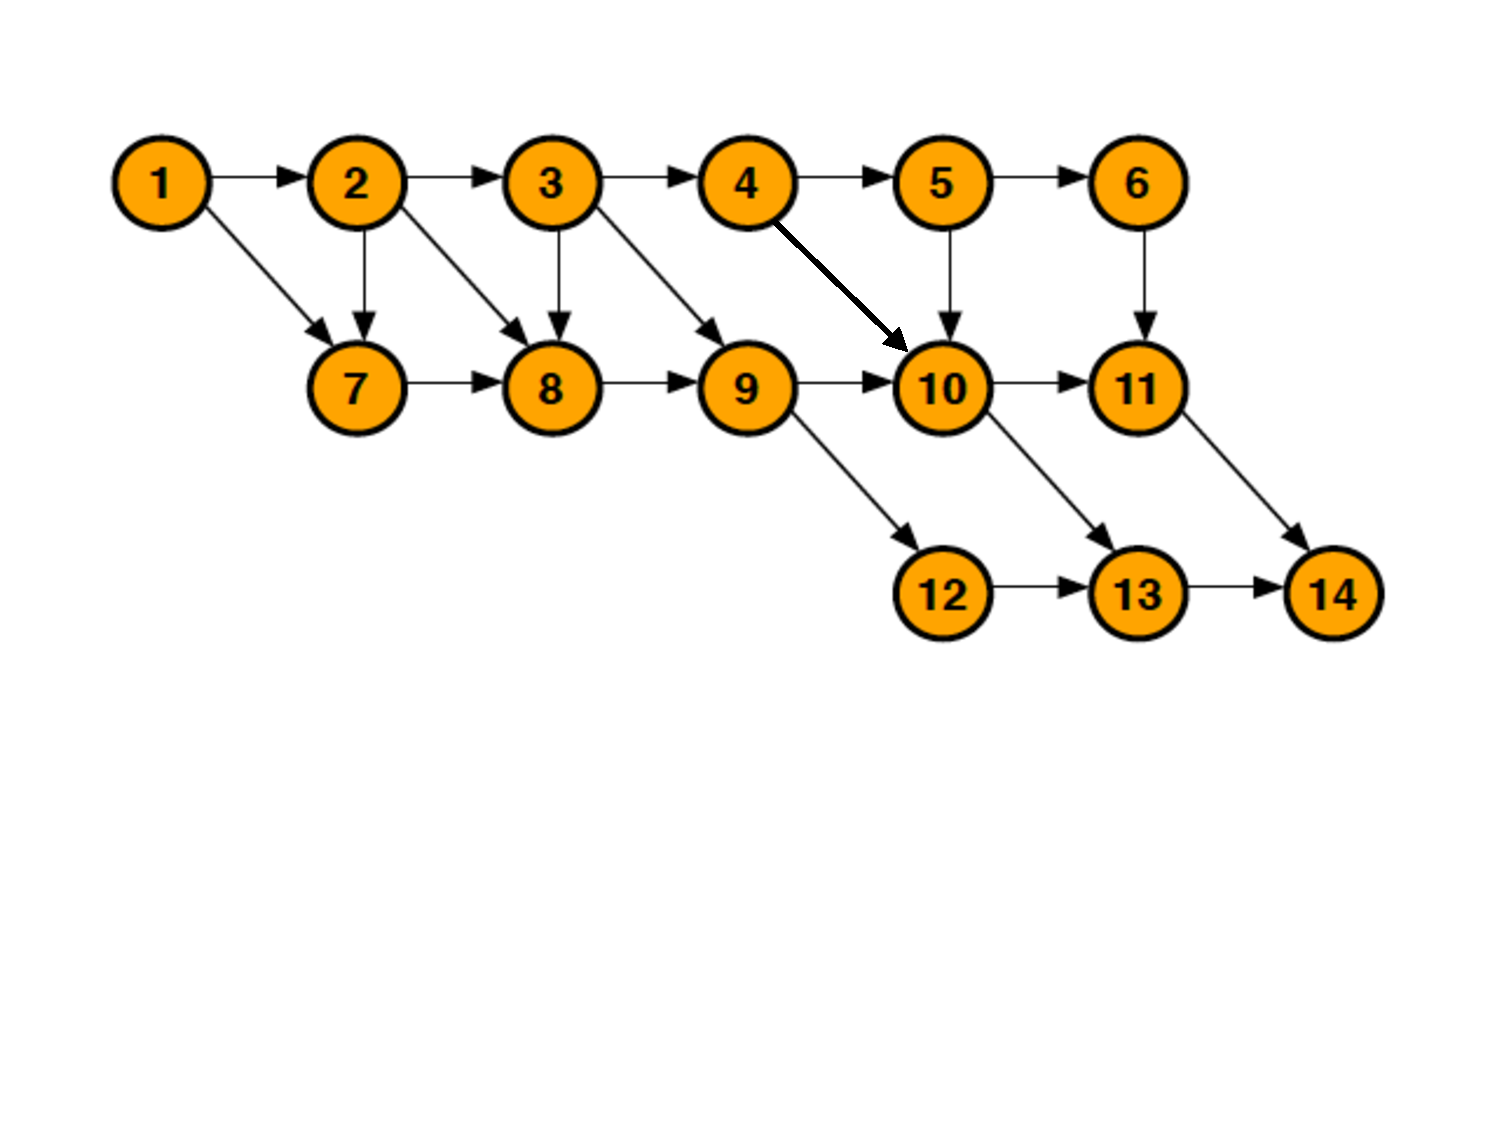
\includegraphics[scale=0.45]{dag_ps10.pdf} 
        \end{center}
        \end{figure}
        % ----------

\end{required}


\begin{proof}[Answer]
%Your answer
\end{proof}




\newpage
\subsection{Problem \ref{Recurrence2}}
\begin{required} \label{Recurrence2}
Suppose we wish to multiply an $n \times m$ and $m \times k$ matrix. This operation takes $nmk$ multiplications. Consider the \textsf{Matrix Product} problem, which defined as follows.
\begin{itemize}
\item \textsf{Instance:} Matrices $A_{1}, \ldots, A_{n}$ with integer entries, where $A_{i}$ has dimensions $n_{i} \times m_{i}$. Note that for $1 \leq i < n$, we necessarily have that $m_{i} = n_{i+1}$.

\item \textsf{Solution:} Compute $A_{1}A_{2} \cdots A_{n}$, using the minimum number of integer multiplications.
\end{itemize}


\noindent \\ We note that matrix multiplication is associative; that is, $A(BC) = (AB)C$. So we may parenthesize $A_{1}A_{2} \cdots A_{n}$ however we wish, without changing the expression. Certain parenthesizations require fewer multiplications than others. For instance, suppose $A$ is a $10 \times 30$ matrix, $B$ is a $30 \times 5$ matrix, and $C$ is a $5 \times 60$ matrix. Observe that $A(BC)$ requires $(10 \cdot 30 \cdot 60) + (30 \cdot 60 \cdot 5) = 27000$ multiplications, while $(AB)C$ requires $(30 \cdot 5 \cdot 10) + (10 \cdot 5 \cdot 60) = 4500$ multiplications. \\

\noindent For $1 \leq i \leq j \leq n$, denote $m[i, j]$ as the minimum number of multiplications required to evaluate $A_{i} \cdots A_{j}$. Note that $m[i, j]$ is given by the following recurrence:
\[
m[i, j] = \begin{cases} 
0 & : i = j, \\
\displaystyle \min_{i \leq k < j} (m[i, k] + m[k+1, j] + n_{i}m_{k}m_{j}) & : i < j.
\end{cases}
\]

\noindent Here, we have that:
\begin{itemize}
\item $m[i, k]$ is the minimum number of multiplications to compute $M_{1} := A_{i} \cdots A_{k}$. Note that $M_{1}$ is an $n_{i} \times m_{k}$ matrix.

\item $m[k+1, j]$ is the minimum number of multiplications to compute $M_{2} := A_{k+1} \cdots A_{j}$. Note that $M_{2}$ is an $m_{k} \times m_{j}$ matrix (here, $m_{k} = n_{k+1}$).

\item $n_{i}m_{k}m_{j}$ is the number of multiplications required to compute $M_{1} \cdot M_{2}$. 
\end{itemize}


\noindent \\ \textbf{Your job} is as follows. Suppose we are given matrices of the following dimension:
\begin{itemize}
\item $A_{1}$: $2 \times 8$.
\item $A_{2}$: $8 \times 9$.
\item $A_{3}$: $9 \times 10$.
\item $A_{4}$: $10 \times 20$.
\item $A_{5}$: $20 \times 6$.
\end{itemize}

\noindent \\ Design and fill in a 2D lookup table to compute the minimum number of integer multiplications required to compute $A_{1} \cdots A_{5}$. Include the optimal back pointers. [\textbf{Note:} You may hand-draw and embed your lookup table, provided it is legible and we do not have to rotate our screens to read it. All other accompanying work \textbf{must} be typed.]
\end{required}

\begin{proof}[Answer]
%Your answer here
\end{proof}

\end{document} % NOTHING AFTER THIS LINE IS PART OF THE DOCUMENT



